\chapter{Assessing Developer Knowledge}
\label{chap:assess}

To create any kind of model, I need a dependent variable and one or more independent variables that could be used to predict the value of the dependent variable. Since I want to build models that predict knowledge, my dependent variable has to be some measure of developer concept knowledge.
Borrowing from existing computer science education research, I developed concept inventories for knowledge assessment. 

A concept inventory, or CI for short, is a validated assessment that uses multiple-choice questions to aid instructors in assessing student understanding of relevant domain or course concepts, while also identifying student misconceptions~\cite{evans2003progress}. Concept inventories can cover any range of concepts and originated in the field of physics with the Force Concept Inventory~\cite{hestenes1992force}. There are guidelines for creating concept inventories, such as avoiding catch-all options like ``All of the above'' and using empirical methods to validate and improve inventory questions and items. Most often in the natural sciences and engineering, inventories assess breadth of knowledge across the subject or course of interest~\cite{evans2003progress}. In Computer Science, for example, a range of CS1 concepts can be represented in a given concept inventory~\cite{tew2010developing}.

% TODO does this need to go to RW?	
Borrowing from concept inventories used in other STEM fields, CS Education researchers and instructors have developed various concept inventories for assessing students' knowledge of introductory Computer Science concepts\cite{almstrum2006concept, krone2010reasoning,tew2010assessing}. Almstrum and colleagues created concept inventories to assess student knowledge of concepts taught in a discrete mathematics course~\cite{almstrum2006concept}. 
Tew and Guzdial developed a concept inventory for assessing students' knowledge of CS1 concepts in introductory Computer Science courses~\cite{tew2010assessing, tew2010developing}. These inventories used textbooks and experts to create test specifications that they then validated using empirical methods, such have CS Education experts review the specification. Fundamental concepts included on their concept inventory include object-oriented programming and control structures. Similar to other Computer Science concept inventories, Tew and Guzdial's CS1 concept inventory assess breadth of knowledge. 
	
Related to the concept inventories developed by Tew and Guzdial, Zingaro and colleagues developed ConcepTests~\cite{zingaro2010experience} used in to monitor and assess student understanding of computer science concepts as they were taught. Similar to my concept inventories, these ConcepTests focus on one specific concept at a time except with the goal of encouraging and implementing peer instruction (PI). In contrast, Zingaro and colleagues do not use the validated steps for creating a concept inventory to create their assessments.
	
Also closely related to my approach and the goal of my inventories is the work of Karpierz and Wolfman, who designed a variety of multiple choice questions for concept inventories on binary search trees and hash tables~\cite{Karpierz2014Misconception}. Rather than focusing on various Computer Science concepts at once, they focus on developing questions to assess specifically binary search trees and hash tables. Contrary to our approach, they only deployed their concept inventory once -- during the last lecture of the course. This eliminates the possibility of comparing how much students knew before taking the course and how much they know now, which I assess with my concept inventories.
	
Although these concept inventories have been proven useful in various contexts, some instructors believe, and research suggests, we should be moving away from textbook-driven lessons and assessments, and employ more focused efforts to monitor student learning and understanding~\cite{pellegrino2001knowing, ghezzi2005challenges, wohlin1999achieving}. This work builds on existing work by adapting current methods used to develop concept inventories by 1) assessing depth of knowledge regarding a single programming concept, 2) using language specification, tutorials, and other technical documents to create the content of the concept inventories, and 3)incorporating practical software engineering concepts, such as tool use.

\section{Modified Concept Inventories}

Traditionally, concept inventories are used to  assess conceptual knowledge across concepts; in Computer Science, the target audience is typically CS1 students~\cite{tew2010developing,kaczmarczyk2010identifying}. 
I wanted to evaluate the potential for a depth versus breadth approach to assessing conceptual knowledge, that incorporates software engineering concepts and practices, with the target audience being developers at any stage of expertise.
Therefore, I could not borrow directly from research that uses a breadth approach to create concept inventories that assess high level knowledge of concepts taught in an introductory course~\cite{tew2010assessing}. I extended existing concept inventory research~\cite{tew2010developing,nelson1967testing} by using the new Bloom's Taxonomy to create questions~\cite{scott2003bloom,thompson2008bloom, starr2008bloom}, subjective resources like language specifications to determine sub-concepts relevant to a single concept, and tool output, including compilation errors and warnings, to integrate practical applications of the programming concepts. The differences between my approach and existing approaches is highlighted in Table~\ref{table:diff}.
The final process we have developed for creating general knowledge programming concept inventories that assess depth of knowledge is as follows:

\begin{enumerate}
    \item Define Conceptual Content for Test Specification
    \item Build Bank of Test Questions
    \item Pilot Questions
    \item Establish Validity and Reliability
\end{enumerate}




	\begin{table}[ht]
		\centering
		\caption{Summary of the differences between my approach and existing approaches.}
		\label{table:diff}
		\rowcolors{2}{gray!25}{white}
		\begin{tabular}{lll}
			\toprule
		    \rowcolor{gray!50}
			& \multicolumn{1}{c}{\textbf{Existing CS Concept Inventories}}                                              & \multicolumn{1}{c}{\textbf{My Concept Inventories}}\\
			\midrule
			\textbf{\begin{tabular}[c]{@{}l@{}}Defining Concept \\Content  for \\ Test Specification\end{tabular}} & \begin{tabular}[c]{@{}l@{}}Textbooks; provide definitions to \\ CSEd experts for review \end{tabular}                                                   & \begin{tabular}[c]{@{}l@{}}language specifications, language \\ tutorials, and documentation\end{tabular}      \\
			\textbf{\begin{tabular}[c]{@{}l@{}}Build Bank of \\Test Questions \end{tabular}}                                                              & \begin{tabular}[c]{@{}l@{}}Three types of questions \\ (Definitional, Tracing, Code Completion)\end{tabular} & \begin{tabular}[c]{@{}l@{}}Six types of questions (Bloom's \\ Taxonomy), tool output, compilation\end{tabular} \\
			\textbf{Pilot Questions}                                                                            & Collect data for later analysis                                                                              & \begin{tabular}[c]{@{}l@{}}Iteratively conduct think aloud\\ and modify \end{tabular}                                                                     \\
			\textbf{\begin{tabular}[c]{@{}l@{}}Establish Validity \\ \& Reliability \end{tabular} }                                                         & Empirical analysis of responses                                                                              & Item and distractor analysis\\  
			\bottomrule
		\end{tabular}
	\end{table}

\section{Defining Conceptual Content}

A test specification is a way of formally outlining what will be on the test without having to write any of the questions~\cite{tew2010developing}. Once a decision has been made concerning the programming language and concept(s) of interest, rather than using expert review to determine appropriate sub-concepts concepts, use a more objective, practical approach. This is achieved by using language specifications, tutorials, and other documentation surrounding that concept. This is an iterative process meant to increase the depth of assessment on the concept and related sub-concepts.

% To better understand how we constructed and validated our concept inventories, let us consider our most recent concept inventories on generics and exception handling.
To determine the conceptual content for each concept inventory, I identified key concepts from the most up to date the Java Language Specification (JLS)~\cite{Gosling:1996:JLS:560667} and the Oracle Java Concept Tutorials\footnote{\url{http://docs.oracle.com/javase/tutorial/java/generics/}} on the concept of interest. The Oracle Java Tutorial was most useful for finding and mapping the relationships between concepts and ancestor concepts; if Lesson X built on top of Lesson Y, we consider Lesson Y an ancestor of Lesson X. For example, based on the generics tutorial, we labeled Upper Bounded Wildcards as an ancestor concept to Wildcards. 

	\begin{figure*}[ht]
		\centering
		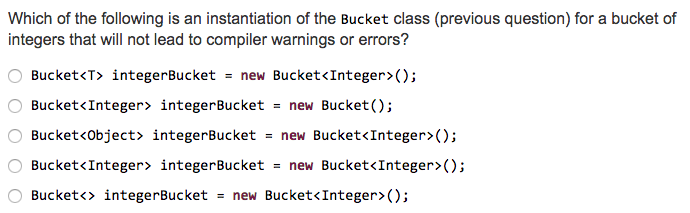
\includegraphics[width=4in]{Chapter-5/figs/generics-Q2.png}
		\caption{Question assessing ability to evaluate generic type instantiation.\label{fig:Q2}}
	\end{figure*}	
	
Once I had a list of concepts and sub-concepts, I created questions to assess the various concepts, mapping each question to at least one level of Bloom's Taxonomy. I used examples found in the language specifications and tutorials, along with relevant tool output, to create questions for each inventory. For example, the item shown in Figure~\ref{fig:Q2} is a question on the generics concept inventory that asks a question to determine the student's ability to \textbf{evaluate} a problem pertaining to instantiating a generic type (\texttt{Bucket}). According to the new Bloom's Taxonomy, evaluation includes Checking and Critiquing, which involves students making decisions based on criteria. In terms of Computer Science, prior works suggests this can be done by, for example, assessing students' ability to determine if a piece of code satisfies requirements (i.e. compilation) or critiquing the quality of the code based on known standards~\cite{thompson2008bloom}.

\section{Building A Bank of Questions}

Based on existing concept inventory research, the questions on concept inventories should be multiple choice and all questions should have the same number of items to choose from~\cite{tew2010developing}; typically there are 4--5 items. Existing work also recommends avoiding catch-all items such as ``All of the above'' and ``None of the above''~\cite{tew2010developing}. While one of the items should be the best right answer, other options, known as distractors, should be plausible permutations that are believable but incorrect. 

Next, using the revised Bloom's Taxonomy, which is the most up to date version of the taxonomy, is to derive a bank of test questions. Using Bloom's Taxonomy increases assurance that the questions assess different levels of understanding, which helps assess mastery of a concept~\cite{scott2003bloom, thompson2008bloom}. Each question should map to at least one level of Bloom's Taxonomy~\cite{starr2008bloom,khairuddin2008application}; rigor increases at each level. I found it helpful to compare the kinds of questions asked at each level of Bloom's Taxonomy with the questions in the bank to be used. I believe it is more effective if each level of Bloom's Taxonomy is represented in the bank of questions at least once rather than only focusing on certain levels of the Taxonomy~\cite{scott2003bloom}. 
To further incorporate practical aspects of software engineering, for each inventory, create questions that ask about code compilation, writing quality code, and resolving tool output. 
% Instructors can use languages and tools of their preference for creating these questions; we believe it is ideal if they are tools instructors plans to or already has introduced to students.

\section{Think Aloud Pilots}
Once there is a bank of questions, the next step is to pilot the questions. The goal of this pilot is to determine if there are any obvious ambiguities in the questions or options. Consistent with Parker and colleagues~\cite{parker2016replication}, we recommend a think-aloud activity where students take each concept inventory and report questions or items that stand out as confusing and why. As participants note ambiguous words or phrases used in the questions or items, immediately make modifications before having any others pilot the inventory. When observing the scores, if all the scores are really high, or really low, this might suggest an assessment that is too difficult or too easy~\cite{nelson1967testing}, which would require revisiting and revising the questions or items. To ensure items contribute to overall effectiveness, use statistical methods to validate the concept inventories.

I piloted my concept inventories with undergraduate and graduate students. For each student, I asked them to take the inventory as they normally would and let us know when one of the following occurs:
	
	\begin{itemize}
		\item They came across a question where the phrasing did not make sense or was unclear.
		\item The came across an option for a question that did not make sense or was unclear.
		\item They encountered a question where they believed more than one option could be correct.
		\item They encountered a question where none of the options appear to be correct.
		\item They noticed any typos or discrepancies in the questions, options, or code examples.
	\end{itemize}
	
I made note during this process of any issues participants encountered, asked them to explain that difficulty, and how it could be improved. Once that participant finished the concept inventory, I immediately integrated the necessary changes into the concept inventory. I iterated this process with all pilot participants.

\section{Concept Inventory Validation}

Validation of an assessment tool can be done in a variety of ways.
To test the validity of my concept inventories and the items on each, I conducted \textit{item analysis} and \textit{distractor analysis} using R statistical software~\cite{boopathiraj2013analysis, RSoftware}. 
I ran these analyses based on data gathered from a different sample than the group used for the initial think aloud pilot. 

\subsection{Item Analysis}
The most common form of validation is item analysis~\cite{gorsuch1997exploratory}.
Item analysis determines if inventory items are valid methods of assessment; most often, the item difficulty and discrimination index are used to assess test quality~\cite{boopathiraj2013analysis}. For item difficulty, an item is considered too easy if its item difficulty value (Item Difficulty, Table~\ref{table:items}) is 0.95--1.00 and too difficult if it is less than 0.20. An optimal question has an item difficulty value of 0.50, however, the primary goal is to not have any questions, based on the item difficulty value, that are too hard or too easy. 

A question is considered satisfactory if the discrimination index (Point Biserial, Table~\ref{table:items}) is greater than 0.20. The difficulty and point biserial values can be positive or negative; a negative value suggests an item should be removed or replaced.
The threshold value (Item Threshold, Table~\ref{table:items}) provides the same information as the difficulty value; the lower the value, the easier the question. 
The biserial value (Biserial, Table~\ref{table:items} describes the degree of relationship between two interval scales. For the type of validation needed for the inventories, the threshold and biserial are not relevant.


To clarify the validation process, I present item analysis results from the exception handling concept inventory as an example. This was the concept inventory that underwent the most change as a result of this process. Table~\ref{table:items} shows the item analysis output from the initial set of exceptions questions put in thee inventory and piloted with 10 students and developers. I wanted to include developers with industry experience to evaluate the more advanced questions on the inventory. I performed pilots with students and those with industry experience to evaluate how well the concept inventory assessed different levels of knowledge regarding exception handling. Based on the output, one of the questions removed was item 3, which is shown in Figure~\ref{fig:item3}. The discrimination index for this item (-0.024) is too low, which means that it was not a good item for discriminating between students who are knowledgeable in exception handling and those who are not. Based on these numbers, I also removed items 4, 8, and 9.

	\begin{table}[]
		\centering
		\caption{Exception handling concept inventory item analysis results}
		\label{table:items}
		\begin{tabular}{lllll}
			\toprule
			& \multicolumn{1}{c}{\textbf{\begin{tabular}[c]{@{}c@{}}Item \\ Difficulty\end{tabular}}} & \multicolumn{1}{c}{\textbf{\begin{tabular}[c]{@{}c@{}}Item \\ Threshold\end{tabular}}} & \multicolumn{1}{c}{\textbf{Point Biserial}} & \multicolumn{1}{c}{\textbf{Biserial}} \\
			\midrule
			\textbf{Item 1}  & 0.917                                                                                   & -1.383                                                                                 & 0.271                                       & 0.489                                 \\
			\textbf{Item 2}  & 0.333                                                                                   & 0.431                                                                                  & 0.098                                       & 0.127                                 \\
			\textbf{Item 3}  & 0.667                                                                                   & -0.431                                                                                 & -0.024                                      & -0.032                                \\
			\textbf{Item 4}  & 0.917                                                                                   & -1.383                                                                                 & 0.271                                       & 0.489                                 \\
			\textbf{Item 5}  & 0.500                                                                                   & 0.000                                                                                  & 0.553                                       & 0.694                                 \\
			\textbf{Item 6}  & 0.500                                                                                   & 0.000                                                                                  & 0.484                                       & 0.607                                 \\
			\textbf{Item 7}  & 0.583                                                                                   & -0.210                                                                                 & 0.690                                       & 0.872                                 \\
			\textbf{Item 8}  & 1.000                                                                                   & -Inf                                                                                   & N/A                                         & N/A                                   \\
			\textbf{Item 9}  & 0.500                                                                                   & 0.000                                                                                  & 0.899                                       & 1.000                                 \\
			\textbf{Item 10} & 0.833                                                                                   & -0.967                                                                                 & 0.495                                       & 0.738                                 \\
			\textbf{Item 11} & 0.500                                                                                   & 0.000                                                                                  & 0.899                                       & 1.000                                 \\
			\textbf{Item 12} & 0.667                                                                                   & -0.431                                                                                 & 0.489                                       & 0.634                                 \\
			\textbf{Item 13} & 0.583                                                                                   & -0.210                                                                                 & 0.690                                       & 0.872                                 \\
			\textbf{Item 14} & 0.667                                                                                   & -0.431                                                                                 & 0.342                                       & 0.444\\                                
			\bottomrule
		\end{tabular}
	\end{table}
	
	
	\begin{figure}[]
		\centering
		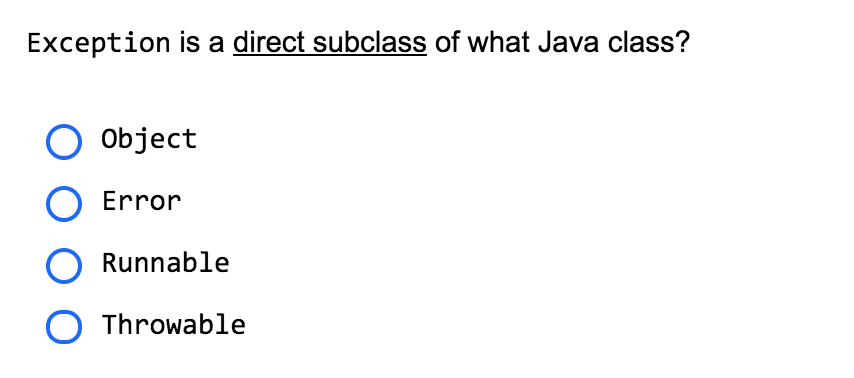
\includegraphics[width=3in]{Chapter-5/figs/item3.png}
		\caption{Item removed from original concept inventory. \label{fig:item3}}
	\end{figure}

\subsection{Distractor Analysis}
I also recommend distractor analysis to evaluate the changes made during the think-aloud piloting. Distractor analysis determines if the options provided for a given question are fair and if the incorrect options contribute to the quality of the inventory. If the incorrect options are nonsensical or would make no sense as the answer, this takes away from the quality of the concept inventory. For example, if the only item that makes sense is the correct response, the chances that students can guess the right response as opposed to knowing the right response is increased.

The goal is for there to be no distractors that are not being selected and for the high performers (middle to upper range) to most often select the correct response. Because this was the case in the data for all the inventories, I kept all response options for each inventory item.\footnote{The final version of the concept inventories can be found at the following urls: \url{http://go.ncsu.edu/null}(null object dereferencing), \url{http://go.ncsu.edu/generics}(generics), \url{http://go.ncsu.edu/exceptions}(exception handling).}
% TODO footnote ==> appendix?
As with previous work, because establishing reliability for one inventory requires data from multiple trials, it may be better to save exploring reliability for future analysis~\cite{tew2010developing,tew2010assessing}.


	
% TODO talk about applications for my inventories?? stuff in paper = education only :/ 
% TODO talk about industry and classroom applications -- end with how I'm using them?


\section{Limitations \& Challenges}\label{sec:limits}

Despite the possibilities for our approach for creating and deploying these concept inventories, there are some limitations. 

\begin{itemize}
	\item \textbf{Upfront time commitment.} Although there is value inside and outside the classroom in the process we proposed for depth of knowledge assessment, there is an upfront time cost involved in creating an inventory using our process. In our experience, after creating the first couple of inventories, especially with the up front cost of understanding how to conduct item analysis and what the results mean, the amount of time it takes to create new inventories decreases.
	\item \textbf{Lack of automation for individual response assessment.} Currently, to our knowledge, there is no automated way to observe individual student responses and changes over time, outside of item analysis. Item analysis, which we performed on pilot data from our concept inventories, provide some insights into the effectiveness of each item on the evaluation. However, it does not ease the process of determining which concepts need more attention in class or lab which is one of the potential uses for our inventories.
	\item \textbf{Guaranteeing student's responses are their own.} Even though we did not deploy our concept inventories for a grade, it is still possible that students used outside sources, or even each other, to help determine answers on the inventory. There is no sure way to guarantee students are not using outside resources. However, we attempted to mitigate this limitation by only allowing so much time for taking the inventory and making it an in class exercise rather than a homework assignment.
	\item \textbf{Keeping concept inventories up to date.} Depending on the language concepts are being taught in, there may be a need to periodically re-assess the material on the inventory for updating. So far, we have not had to make any updates however generics and exception handling are great examples of language features that has evolved since it has been out. Because our concept inventories aim to achieve depth of knowledge assessment, it is important that all relevant sub-concepts are represented in the inventory.
	\item \textbf{Lack of student participation.} Because the exercise is not graded, and in short our concept inventories are specialized quizzes, students may not be enthusiastic about having to take them. The hope is that, however, students who are genuinely interested in the coursework and progressing will take the inventories seriously whether they are enthusiastic about it or not.
	\item \textbf{Deploying the same concept inventory twice.} When deploying our concept inventories, we provided students with the same inventory as their pre- and post-evaluation and, if interested, they could continue past the end of the inventory to see which responses they got correct or incorrect. This introduces the potential that students are learning from the concept inventory rather than the lectures. Although we are unsure of how many students looked at what they got right and wrong, we argue that it is not a disadvantage for students to learn from the concept inventory. Because we use very few definition questions on our inventories, students are given access to practical problems and solutions that can benefit them in the future. 
\end{itemize}